% !TeX root = ./main.tex
% !TeX spellcheck = en-GB

% Font size
\documentclass[12pt,a4paper,british]{report}

\usepackage{ifxetex}

\ifxetex
  \usepackage{fontspec}
\else
  \usepackage[T1]{fontenc}
  \usepackage[utf8]{inputenc}
  \usepackage{babel}
  \usepackage{lmodern}
\fi

\usepackage[margin=1in]{geometry}

\usepackage{hyperref}

% license
\usepackage[
    type={CC},
    modifier={by-nc-sa},
    version={4.0},
]{doclicense}

\usepackage{appendix}

% prevent floating figures 
\usepackage{float}

\usepackage{graphicx}

\usepackage[justification=centering]{caption}

% Referencing
\usepackage[backend=biber,bibstyle=apa,citestyle=authoryear]{biblatex}

\addbibresource{document-visualizations.bib}

% break bilbatex reference URL on number
\setcounter{biburlnumpenalty}{9000}

% packages for Header and Footer
\usepackage{lastpage}
\usepackage{fancyhdr} 
 
%----------------------------------------------------------------------------------------
%	TITLE SECTION
%----------------------------------------------------------------------------------------

\title{\textbf{High level document visualisation}}

\author{\textit{guillaumedsde}}

 % Date, use \date{} for no date
\date{\today}

% save these variables for later use under different name
\makeatletter
\let\doctitle\@title
\let\docauthor\@author
\let\docdate\@date
\makeatother

%----------------------------------------------------------------------------------------
%	HEADER AND FOOTER SECTION
%----------------------------------------------------------------------------------------
\pagestyle{fancy}

% sets both header and footer to nothing
\fancyhf{}

% Header
% remove horizontal header bar
\renewcommand{\headrulewidth}{0pt}
% left hand side header
\lhead{\doctitle}
% right hand side header
\rhead{\docauthor}
\setlength{\headheight}{15pt}

% Footer
% center of footer
\cfoot{\thepage\ of \pageref{LastPage}}


%------------------------------------------------------------------------

\begin{document}

% Print the title section
\maketitle

I have a Kindle, I read many books, not always to completion and being able to ``carry'' all of them in one device rather than each as physical objects is a godsend. I can also search through the book's text to easily go back and find a particular quote.

For all these comforts however, I sacrifice being able to \textit{flick} through pages of a book. Quickly ``overviewing'' text with such precise granularity has yet to be mimicked by any computer ``scrolling'' input. Scrolling on a touch screen with a finger lacks any feedback, a mouse scroll wheel does have feedback with each ``notch'', which can be perfected to have \href{https://www.theverge.com/circuitbreaker/2019/10/29/20937114/logitech-mx-master-3-mouse-wheel-hardware-scroll-button}{impressive tactile feedback} that ``disengages'' as one scrolls faster.

However, nothing compares to the granularity and control of human fingers flicking through pages for an overview of paged text. Given the increasing amounts of data generated, a ``high level'' overview of documents comparable to flicking through pages and better than a scroll wheel becomes increasingly useful for ``Navigating and viewing large information spaces'' \autocite{bartramContinuousZoomConstrained1995}.

\section*{Document body outline with emphasis as overview thumbnails}

There are quite a few ``document thumbnails'' that abstract textual content away and keep line length for displaying document overviews, much like many modern text editors. Adding emphasis on gray line representation of text lines provides for a good overview of document content and feature `location' in the document, but it does not convey much information beyond that, see Figure \ref{fig:j24}.

\begin{figure}[H]
  \centering
  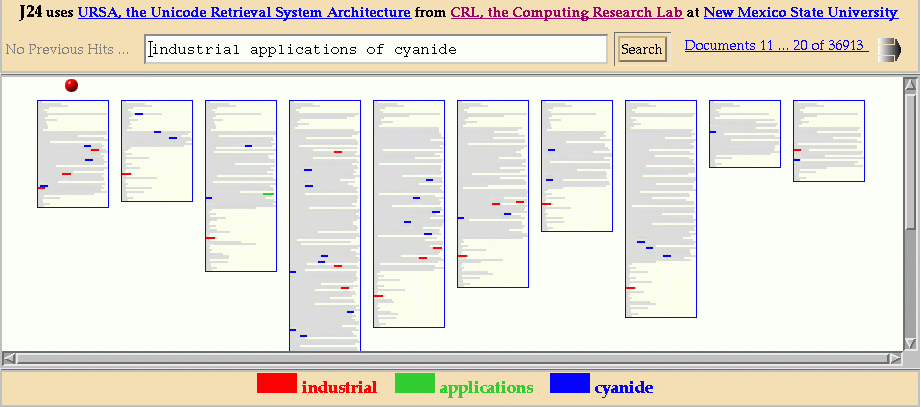
\includegraphics[width=\textwidth]{static/j24.png}
  \caption{``J24'' software's document overview with feature highlighting \\ \protect\autocite{ogdenDocumentThumbnailVisualizations1998a}}
  \label{fig:j24}
\end{figure}

\section*{Lexical Episode Plots}

A variation of this kind of document overview displays highlights beside the document outline also showing the ``topic'' of the highlight, it is called ``Lexical Episode Plots'' \autocite{el-assadyVisArgueVisualText2016,goldExploratoryTextAnalysis2015}.

\begin{figure}[H]
  \centering
  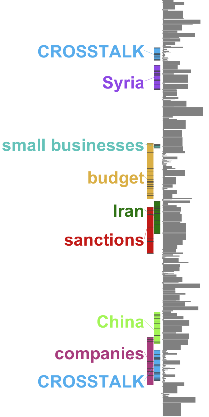
\includegraphics[height=0.5\textwidth]{static/topic-overview.png}
  \caption{``Lexical Episode Plots''\\ \protect\autocite{goldExploratoryTextAnalysis2015}}
  \label{fig:j24}
\end{figure}

\section*{Playing with font size}

\textcite{stoffelDocumentThumbnailsVariable2012} implement a combination of text highlighting along with font size variations for creating distorted thumbnails for previewing important document features.
I am a bit sceptical as to whether this would be a good thumbnail, the highlighted portions definitely show where key features are in the document, but the font size change does not contribute much at the document scale: most words are too small to be legible.
\textit{However} varying font size would be an interesting visualization for the Lime explanation's feature importance.

\begin{figure}[H]
  \centering
  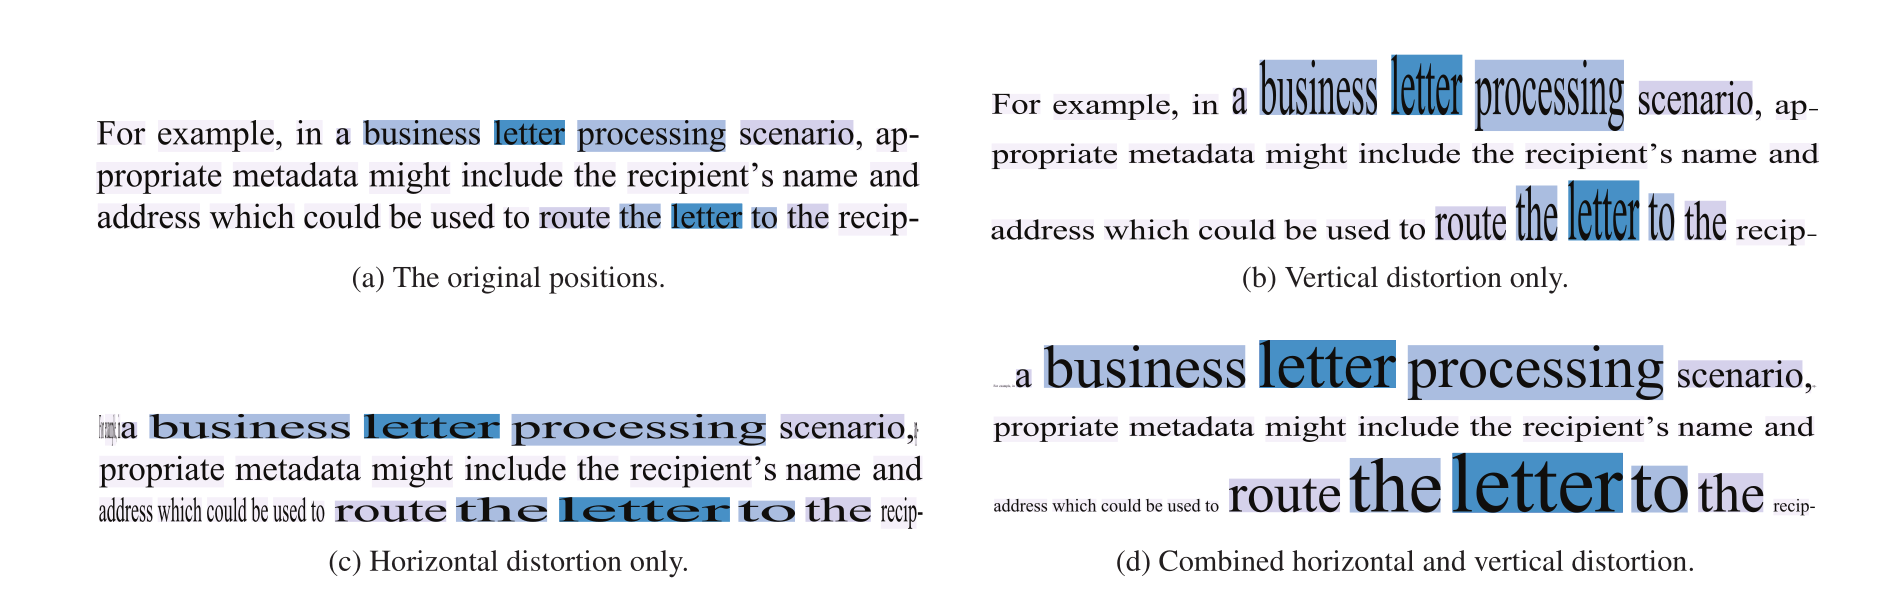
\includegraphics[width=\textwidth]{static/font-size.png}
  \caption{Adjusting font size for overview of important features \\ \protect\autocite{stoffelDocumentThumbnailsVariable2012}}
  \label{fig:font-size}
\end{figure}


\section*{Distortion}

This technique has many names and variants ``Document Lens'' \autocite{robertsonDocumentLens1993}, ``Fisheye'' view \autocite{greenbergFisheyeTextEditor1996} or ``hybrid continuous zoom`` \autocite{bartramContinuousZoomConstrained1995} with different implementations (see Figure \ref{fig:fisheyes}) they are part of a concept called ``Bifocal Display'' \autocite{apperleyBifocalDisplay}.

\begin{figure}[H]
  \centering
  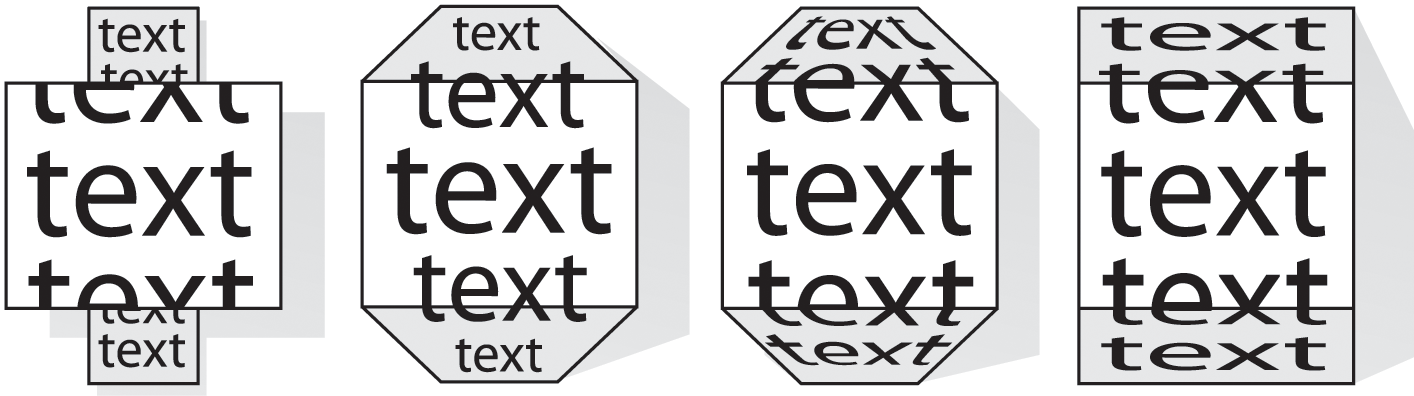
\includegraphics[width=\textwidth]{static/different-fisheyes.png}
  \caption{Different Fisheye views, from left to right: \\ Manhattan lens, zoomscapes, central perspective and parallel projection \\ \protect\autocite{baudischFishnetFisheyeWeb2004}}
  \label{fig:fisheyes}
\end{figure}

\textit{Circular Fisheye Distortion} is a circular ``magnifying glass'' effect visible in \textcite{bostockFisheyeGrid2019}. \textit{Cartesian Distortion} ``magnifies continuously so as to avoid local minification'' \autocite{bostockFisheyeDistortion2012}. The effect can also be limited to only one axis (vertical or horizontal) as seen in \textcite{pstuffaCartesianFisheyeDistortion2019}. In our case, Vertical Cartesian Distortion on a per line basis seems like an interesting visualization for document overview with emphasis on hovered lines. There is a D3js implementation of this effect (see the links above), it also seems like there is a React specific implementation of this text fisheye effect \autocite{zhongVincentdchanReactfisheye2019}.



%----------------------------------------------------------------------------------------
%	BIBLIOGRAPHY
%----------------------------------------------------------------------------------------

\newpage

% \emergencystretch=1em

\section*{References}

\printbibliography[heading=none]

\vspace*{\fill}
% print license
% \doclicenseThis

\end{document}
